\subsection{Completeness Properties of (TO)HTN Planners}
In our presentation on different search algorithms implemented in CrowdHTN we already did a short discussion on the completeness of different algorithms in section \ref{improv: search completeness}. The current section will start with a short recap of our findings, expand them to other planners and will then do an expanded discussion that takes factors like loop detection and restarts into account. \\
Before we dive into the more detailed discussion we want to note that we have seen in section \ref{prelim: tohtn complexity} that there is an upper bound to task network depth where if a plan exists there always exists a plan up to that depth. By limiting our planning to task network expansions with lower depth, we can trivially achieve completeness. This is however of little practical use as this depth bound is exponential in the problem size. As a result, we can expect to run out of memory before hitting this bound. For this reason we do not make use of this bound and as far as we know no other planner does it either. We will now resume a more practical discussion of planner completeness.\\ 
As previously noted, we can split our search algorithms into three main groups:
\begin{itemize}
	\item Algorithms that are complete (BFS, A-star like search)
	\item Algorithms with a chance to find a plan (DFS)
	\item Algorithms which for some domains will never find a plan (heuristic search)
\end{itemize}
\paragraph{Completeness in other planners}
So far we have only classified the different search algorithms present in CrowdHTN. For now we will take a look at other planners, starting with translation-based planners totSAT (\cite{behnke2018totsat}), Tree-REX (\cite{schreiber2019tree}) and Lilotane (\cite{schreiber2021lilotane}). As we have noted in the discussion on planning algorithms in section \ref{prelim: translation based planners}, all three of these planners are based on SAT. Additionally, they all explore the set of potential expansions of the task hierarchy in a layer-by-layer fashion, leading to a BFS-like characteristic in their behavior. As a result, these planners are complete as they are. \\
In contrast to this, we have the space of search-based planners and will take a short look at both HyperTensioN (\cite{magnaguagno2020hypertension}) and PANDA (\cite{holler2020htn}). For HyperTensioN, the authors themselves note that their inbuilt loop detection mechanism suffers from false-positives \cite{magnaguagno2020hypertension}. It follows that their planner is not complete. If we disabled the loop detection in HyperTensioN we would be left with a planner performing DFS, which would put it in the category of planners which are not complete but still have a chance to solve any instance. PANDA on the other hand is a planner based on heuristic progression search, similar to CrowdHTN with our new heuristic. As a result, we expect there to be instances which are impossible to solve. However, PANDA also contains a number of loop detection mechanisms described in \cite{holler2021loop} which in some configurations does not have false positives.

\paragraph{Loop detection and completeness}
As we have seen, heuristic search on its own may increase planner performance but comes at the cost of completeness. We will now explore the implications of combining heuristic search with loop detection to see how this changes the overall situation. In this paragraph we are only interested in loop detection mechanisms that do not suffer from false positives as this automatically disqualifies a planner from being complete. \\


\paragraph{Restarts and completeness}

- restarts solve the problem for DFS
- but only if we get some additional properties!
- i.e. we expect an infinite number of restarts
- additionally, we get an infinite number of runs longer than $t$ seconds for any $t$

- this is nice and gives completeness (yay!)

- loop detection also helps
- loop detection specifically helps if the wrong path is recursive
- warning: recursive does not just mean that we resolve to the same task
- two cases:
	- resolve to same task, but world state is changing
		- i.e., we get the exact same open tasks
		- or in case of HTN we get the same open tasks and a subset of possible orderings to what we had before
		- this will not immediately be detected
		- however, the number of possible world states is bound
		- so eventually we will find the loop, but it will take time
	- resolve to the same task but also add more tasks afterwards ()
		- now the open tasks are different and it is not the same search node anymore
		- oh, look, an example domain
		- the number of open tasks is unbounded
- heuristics cannot be saved via loop detection
- show an example domain with problems! (i.e. search nodes are not identical if we introduce additional open tasks)


- previous section \ref{improv: search completeness} talked about the completeness of different search paradigms

- Lilotane is complete (BFS-like)
- BFS search is complete
- A-star like search is complete

- we could always achieve trivial completeness, but it is not interesting from a practical perspective

- DFS and heuristic search are problematic
- DFS always has a chance to find the right path, but we have to actually hit it
- heuristic search may deterministically take the wrong way

\begin{figure}
	\caption{Pathological instance for our proposed heuristic that is not caught by loop detection}
	\label{figure: pathological heuristic loop}
	\centering
	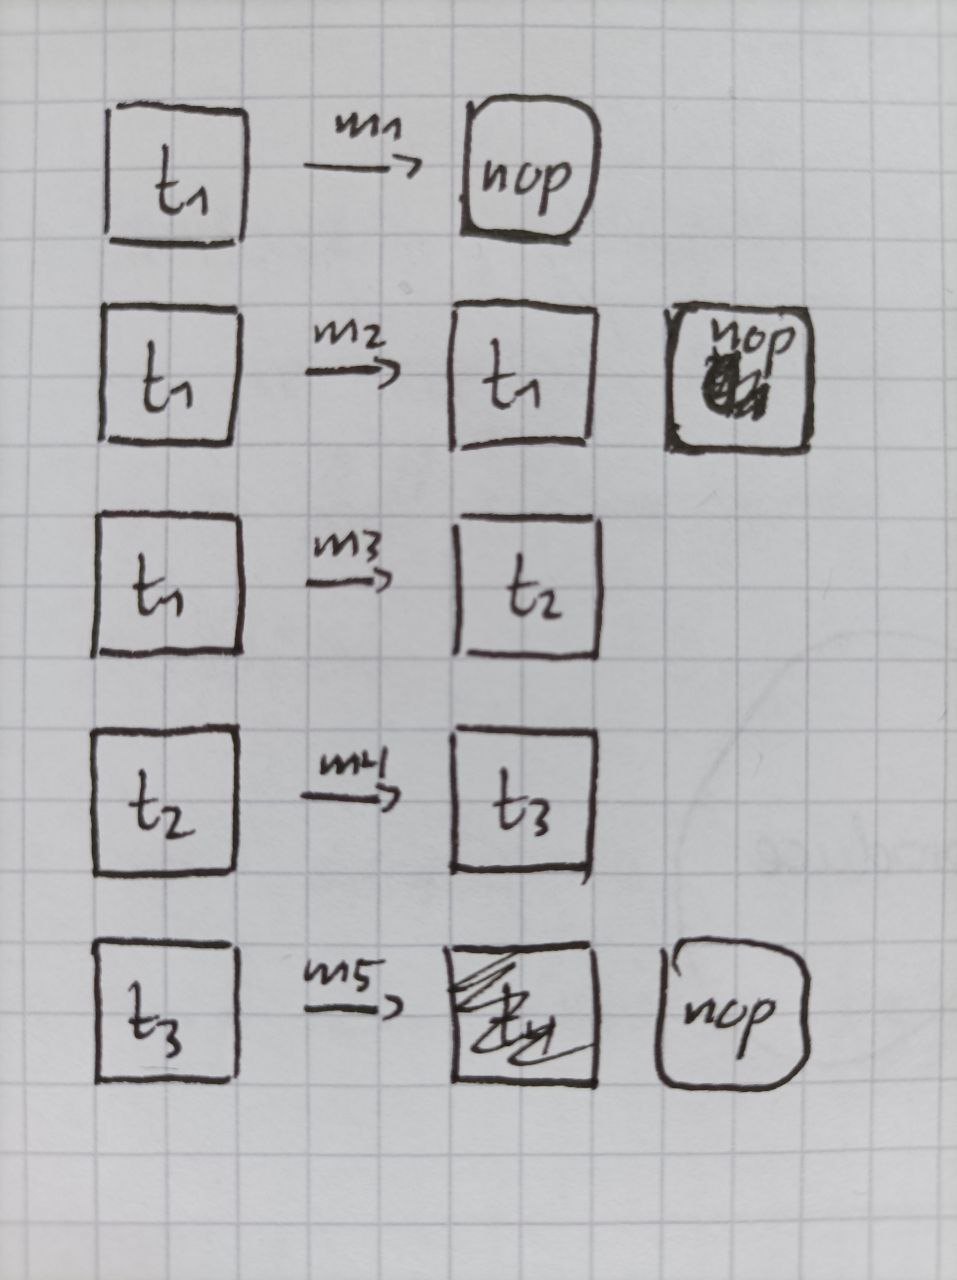
\includegraphics[width=0.3\textwidth]{images/prelim/loop_detection_pathological}
\end{figure}